% MplTplt - Yet another LaTeX template for Modern Physics Lab, PKU.
% Copyright (C) 2014 Huang Kangjing and contributors
 
% This work is completely rewritten basing on the work of Cao Chuanwu
% and Sun Sibai, with texts in the template originally coming from the
% Modren Phys. Lab.
 
% This file is released under the MIT license.
%
% Permission is hereby granted, free of charge, to any person obtaining a copy
% of this software and associated documentation files (the "Software"), to deal
% in the Software without restriction, including without limitation the rights
% to use, copy, modify, merge, publish, distribute, sublicense, and/or sell
% copies of the Software, and to permit persons to whom the Software is
% furnished to do so, subject to the following conditions:
% 
% The above copyright notice and this permission notice shall be included in
% all copies or substantial portions of the Software.
% 
% THE SOFTWARE IS PROVIDED "AS IS", WITHOUT WARRANTY OF ANY KIND, EXPRESS OR
% IMPLIED, INCLUDING BUT NOT LIMITED TO THE WARRANTIES OF MERCHANTABILITY,
% FITNESS FOR A PARTICULAR PURPOSE AND NONINFRINGEMENT. IN NO EVENT SHALL THE
% AUTHORS OR COPYRIGHT HOLDERS BE LIABLE FOR ANY CLAIM, DAMAGES OR OTHER
% LIABILITY, WHETHER IN AN ACTION OF CONTRACT, TORT OR OTHERWISE, ARISING FROM,
% OUT OF OR IN CONNECTION WITH THE SOFTWARE OR THE USE OR OTHER DEALINGS IN
% THE SOFTWARE.
%
 
% This template depends on the "revtex4.1" package from APS Journals
% <http://publish.aps.org/revtex/revtex-faq>, and the Chinese handling
% is done with XeLaTeX engine and package "xeCJK". Please ensure these
% packages are available in your chosen Tex software distribution.
 
% Document created using this template should be compiled with XeLaTeX
% engines rather than plain LaTeX or plain TeX engines.
 
% The non-ASCII texts of this template is encoded in UTF-8 encoding.
% Please note that XeLaTeX only accepts UTF-8 encoded documents, so
% set your editor to use UTF-8 while creating documents with this template.
 
% Recommended TeX software distribution to use with this template is
% Tex Live developed by the TeX User Group (TUG), please visit the home
% page of the distribution <https://www.tug.org/texlive/> for further details.
 
% NOTE THAT IMPORTANT INSTRUCTIONS HAS BEEN WRITTEN AS UPPERCASE COMMENTS
% IN THE TEXT, PLEASE READ THEM CAREFULLY AND FOLLOW THEM TO MAKE THE
% TEMPLATE WORK!
 
% Any further contributions to the template is welcome, please send
% pull requests through github or send mail to maintainer.
 
% For any other questions, please do not hesitate to contact maintainer.
 
% Current maintainer:
% Huang Kangjing <huangkangjing@gmail.com>
 
% Contributors:
% Sun Sibai <niasw@pku.edu.cn>
% Cao Chuanwu <>
% Huang Kangjing <huangkangjing@gmail.com>
 
 
\documentclass[aps,pre,12pt,preprint,onecolumn,showpacs,showkeys]{revtex4-1}
 
% Setting up Chinese handling.
\usepackage{fontspec,xeCJK}
 
% Setting up fonts.
% PLEASE MODIFY ALL THESE FONT NAMES ACCORDING TO YOUR FONT
% INSTALLATION AND PERFERENCE.
 
% Setting up main fonts and mono fonts.
\setmainfont{Liberation Serif}
\setmonofont{Liberation Mono}
% SimSun is required font for the main body of the text.
\setCJKmainfont[AutoFakeBold=5,AutoFakeSlant]{SimSun}
\setCJKmonofont[AutoFakeBold=2,AutoFakeSlant]{SimHei}
 
% Setting up alternative font families.
% Note that these three fonts below are required fonts in document
% title, section headings and figure captions.
\newCJKfontfamily\heiti[AutoFakeBold=2,AutoFakeSlant]{SimHei}
\newCJKfontfamily\fangsong[AutoFakeBold=5,AutoFakeSlant]{FangSong}
\newCJKfontfamily\kaiti[AutoFakeBold=5,AutoFakeSlant]{KaiTi}
 
% Setting up paragraph indent.
\parindent 2em
 
% Setting up macros for Chinese-style font size setting.
\newcommand{\fseight}{\fontsize{5.02}{6.02}\selectfont}
\newcommand{\fsseven}{\fontsize{5.52}{6.62}\selectfont}
\newcommand{\fsssix}{\fontsize{6.52}{7.83}\selectfont}
\newcommand{\fssix}{\fontsize{7.53}{9.03}\selectfont}
\newcommand{\fssfive}{\fontsize{9.03}{10.84}\selectfont}
\newcommand{\fsfive}{\fontsize{10.54}{12.65}\selectfont}
\newcommand{\fssfour}{\fontsize{12.05}{14.45}\selectfont}
\newcommand{\fsfour}{\fontsize{14.05}{16.86}\selectfont}
\newcommand{\fssthree}{\fontsize{15.06}{18.07}\selectfont}
\newcommand{\fsthree}{\fontsize{16.06}{19.27}\selectfont}
\newcommand{\fsstwo}{\fontsize{18.07}{21.68}\selectfont}
\newcommand{\fstwo}{\fontsize{22.08}{26.50}\selectfont}
\newcommand{\fssone}{\fontsize{24.09}{28.91}\selectfont}
\newcommand{\fsone}{\fontsize{26.10}{31.32}\selectfont}
\newcommand{\fsszero}{\fontsize{36.14}{43.36}\selectfont}
\newcommand{\fszero}{\fontsize{42.16}{50.59}\selectfont}
 
% Replace words to Chinese corespondence.
\renewcommand\appendixname{附录}
\renewcommand\abstractname{}
\renewcommand\tablename{表}
\renewcommand\figurename{图}
 
% Replace words in revtex4-1 to Chinese corespondence.
\makeatletter
\def\@pacs@name{\heiti\fssfour \textbf{PACS码:}\normalfont}
\def\@keys@name{\heiti\fssfour \textbf{关键词:}\normalfont}
\def\Dated@name{日期:}
\def\Received@name{\fssfive 接收 }
\def\Revised@name{\fssfive 修订 }
\def\Accepted@name{\fssfive 采纳 }
\def\Published@name{\fssfive 发表 }
\makeatother
 
% Change label style of enumerate.
\renewcommand{\labelenumi}{\alph{enumi}.}
 
% Setting up geometry.
\usepackage{geometry}
\geometry{top=2.54cm,bottom=2.54cm,left=3cm,right=3cm}
 
% Setting up line space.
\usepackage{setspace}
\linespread{1.6}
 
% Setting up hyperreferences.
\usepackage{hyperref}
\hypersetup{colorlinks=true}
 
% Setting up styles for section headings.
\usepackage{titlesec}
\titleformat*{\section}{\bf\fangsong\fsfour}
\titleformat*{\subsection}{\bf\fangsong}
 
% Loading packages for image handling.
\usepackage{subfig}
\usepackage{graphicx,psfrag,epsfig}
 
% Setting up caption styles.
\usepackage{caption}
\DeclareCaptionFont{kaiti}{\kaiti}
\DeclareCaptionFont{bfheiti}{\bf\heiti}
\captionsetup{font=small,format=plain,labelfont=bfheiti,%
  textfont=kaiti,justification=raggedright,%
  singlelinecheck=false}
 
% Loading packages for math typings.
\usepackage{amsmath,amsfonts,amssymb,amsthm,bm,upgreek}
\usepackage[mathscr]{eucal}
\usepackage{siunitx}

\usepackage{listings,xcolor}
\lstset{%
    basicstyle=\footnotesize\fontspec{Liberation Mono},
    keywordstyle=\color{blue}\fontspec{Liberation Mono Bold},
    stringstyle=\color{red}\fontspec{Liberation Mono Bold},
    rulecolor=\color{black},
    numbers=left,
    showspaces=false,
    showstringspaces=false,
    frame=single
}

 
\begin{document}
 
% Title and author info.
\title{\bf\heiti\fsthree X射线标识谱与吸收\vspace{15mm}}
\author{\fangsong\fsfour 黄康靖\vspace{2mm}}
\affiliation{\normalfont\fssfour 北京大学2012级本科生~学号:{masked student id}\vspace{2mm}}
\date{\today}
\keywords{X射线,吸收,标识谱,多道分析器}
\email{huangkangjing@gmail.com; {masked phone number}}
 
% Abstract.
\begin{abstract}
  \vspace{10mm}
  \begin{spacing}{1.5}
    \fssfour
    当原子的外层电子向内壳层上的空位跃迁时,会放出X射线光子.对于不同的原子,因为其
    电子壳层结构的不同,其放出的X射线光子的频率谱是不同的.这一频率谱可以用来唯一
    地标识和测量某一种特定的元素,被称为X射线的标识谱.在今天X射线标识谱技术已经被广泛地用于
    各个领域的技术之中.本实验通过验证性实验,证明了X射线标识谱和对应谱的原子的原
    子序数之间的关系-莫塞莱定律,并且对于X射线与物质的相互作用引发的吸收效应做了
    研究.
  \end{spacing}
\end{abstract}
 
% The main body of the document goes from here.
\maketitle
\fssfour
\section{引言}

\subsection{背景}

1895年德国物理学家伦琴在研究阴极射线时发现了一种新的射线,它不能使用肉眼观察到,
但是可以使铂氰化钡的荧光屏发出荧光.当时伦琴将这一新射线称为X射线.后来为了纪念这
一射线的发现者,也将它称为伦琴射线.

X射线具有直线传播,经过电场不产生偏转,并且穿透力很强的特征.在其发现后不久,它就被
医学界用作检查人体伤病的工具,并用来检查金属或者其他物件内部的缺陷.1912年劳厄等人
研究了X射线在晶体上的衍射现象,证明了X射线本质上是一种电磁波,波长在\SI{0.1}{nm}左右.
1913-1914年莫塞莱发现了元素发出的标识X射线能量与原子序数之间的关系,即莫塞莱定律.
利用莫塞莱定律,1923年人们发现了元素铪.随着闪烁计数器,硅探测器等X射线能谱测量仪器
的发展,利用标识X射线来确定材料的化学组成已经广泛地应用于各种现代谱仪分析技术中.

由于X射线的这些优越的特性与广泛的应用,对于X射线的标识谱所满足的物理规律和X射线与
物质相互作用所满足的物理规律的研究自然具有实在意义.本实验从这个出发点出发,验证了
X射线标识谱所遵守的莫塞莱定律,并且尝试研究了固体对于X射线的吸收过程的相关规律.

\subsection{原理}

\subsubsection{X射线标识谱}

原子的内壳层上存在一个电子的空位时,处于较外层的电子将跃迁入内层以填充这个空位,从
而使得整个原子系统的总能量降低而趋于稳定.根据玻尔的原子理论,外层电子向内层跃迁时,
会发生光辐射,其能量为
\begin{equation}
    \label{eq:Eofphoton}
    h\nu = \frac{2\pi^2m_ee^4}{h^2}(Z - \sigma)^2(\frac{1}{n_1^2} -
    \frac{1}{n_2^2})
\end{equation}
显然,不同原子所辐射出来的荧光光子能量与该原子的能级结构有关,实际上,由于不同种类
的原子的能级结构差别足够大,一旦知道X射线荧光的光子能量,我们就可以断定它来自于哪
一种原子.因此X射线荧光被称为特征X射线,意指为某种原子所持有.

1913-1914年莫塞莱发现,当X射线管中的阳极材料的原子序数$Z$逐渐增加时,相应同一线系
的标识X射线的波长逐渐减小,这种波长的变化是单调地逐渐降低,而不像元素的其他性质那
样具有周期性.他还发现阳极材料的标识X射线频率的平方根和原子序数$Z$之间存在线性关
系,即:
\begin{equation}
    \label{eq:law}
    \sqrt{\nu} = K(Z - \sigma)
\end{equation}
上式称为莫塞莱定律,式中$K$与$\sigma$都是常数,与式~\ref{eq:Eofphoton}相互比较可以
得到常数:
\begin{equation}
    K = \left[\frac{2\pi^2me^4}{h^3}\left(\frac{1}{n_1^2} -
            \frac{1}{n_2^2}\right)\right]^{\frac{1}{2}}
\end{equation}

\subsection{X射线的吸收}

一束强度为$I_0$,光子能量单一的X射线垂直入射到吸收介质上,由于和吸收介质中原子的相
互作用,出射的X射线强度会衰减.当介质厚度很薄时,入射X射线束的强度的相对减少量与吸
收层厚度成正比:
\begin{equation}
    \label{eq:dII}
    \frac{dI}{I} = - \mu_0 dx
\end{equation}
比例常数$\mu_0$称为线衰减系数.

对于X射线来说,线衰减的主要原因是由于线吸收效应(与吸收介质之间发生的光电效应、康
普顿散射和正负电子对产生),而不是弹性散射.并且当X光子的能量在几十\si{keV}时,最主
要的相互作用是光电效应,于是有
\begin{equation}
    \mu_0 \approx \tau_{\text{absorption}} \approx \tau_e
\end{equation}
在式~\ref{eq:dII}上积分得到
\begin{equation}
    \label{eq:II0}
    I = I_0 \exp( - \tau_e x)
\end{equation}
设$\rho$是吸收介质的密度,则式~\ref{eq:II0}可以改写为
\begin{equation}
    I = I_0\exp[-(\tau_e/\rho)\rho x] = I_0\exp(-\tau_m\rho x)
\end{equation}
式中$\tau_m$称为相应于光电效应的质量吸收系数,实际工作中采用此式更为方便.

考虑到原子散射光子的具体过程,应有关系
\begin{equation}
    \tau_m \propto \frac{Z^4}{A}\lambda^3
\end{equation}

\section{实验}

本实验使用X射线照射样品,使得样品原子的内层电子被激发或者电离,形成空位,所使用的激
发源为$^{238}\text{Pu}$衰变过程中所产生的X射线.光子的能量使用硅探测器和微机多
道分析器测量.具体的实验装置示意图如图~\ref{fig:ins}所示.

\begin{figure}[htbp]
  \centering
\includegraphics[width=.3\textwidth]{drawing.pdf}
\caption{\label{fig:ins}%
    实验装置的示意框图;放射源放射出的X射线轰击在样品上,产生的特征X射线被探测器捕
    捉后由多道分析器分析.
}
\end{figure}

为了防止在实验过程中可能出现的中子泄漏,整个装置被包在一个石蜡罐内,唯留一个开口用
来替换样品和吸收片.

实验先后测量了钼、锆、锶、硒、锌、铜、镍、钴、铁和钛样品的K线系X射线标识谱,用于验证莫
塞莱定律.随后又测量了不同厚度的铝片对钼、锆、锌、镍和铁元素的K线系X射线标识谱的
质量吸收系数.

\section{实验结果及分析讨论}

\subsection{莫塞莱定律的验证}

对于莫塞莱定律的验证实验,测量结果数据如表~\ref{tab:data1}所示.

\begin{table}[htbp]
  \caption{\label{tab:data1}
      莫塞莱定律的验证实验的测量结果表.表中的峰位和半峰宽度都是使用道数为单位表
      达的.因为道数与能量之间的线性关系,采用道数作为能量的单位不会影响对于莫塞莱
      定律中线性关系的判断.
  }
\begin{ruledtabular}
  \begin{tabular}{llll}
      样品名称 & 样品原子序数 $Z$ & 峰位置 & 半峰宽度(FWHM) \\
    \colrule
    Mo & 42 & 1965.27 & 33.759 \\
    Zr & 40 & 1768.45 & 32.873 \\
    Sr & 38 & 1598.91 & 47.6574 \\
    Se & 34 & 1265.88 & 33.7234 \\
    Zn & 30 & 963.36 & 33.4109 \\
    Cu & 29 & 898.73 & 34.2512 \\
    Ni & 28 & 839.78 & 44.6599 \\
    Co & 27 & 774.67 & 31.6023 \\
    Fe & 26 & 715.80 & 28.8388 \\
    Ti & 22 & 507.16 & 28.0566
\end{tabular}
\end{ruledtabular}
\end{table}
 
由莫塞莱定律式~\ref{eq:law},以及普朗克关系$E = h\nu$和能量$E$与多道分析器道数$N$之间的
线性关系,可以得到如下关系:
\begin{equation}
    \label{eq:relation}
    N = p_0(Z - p_1)^2 + p_3
\end{equation}

对于表~\ref{tab:data1}中测得的实验结果,按照式~\ref{eq:relation}的形式对其进行拟
合,得到的结果绘制成曲线,见图~\ref{fig:res}.


\begin{figure}[htbp]
  \centering
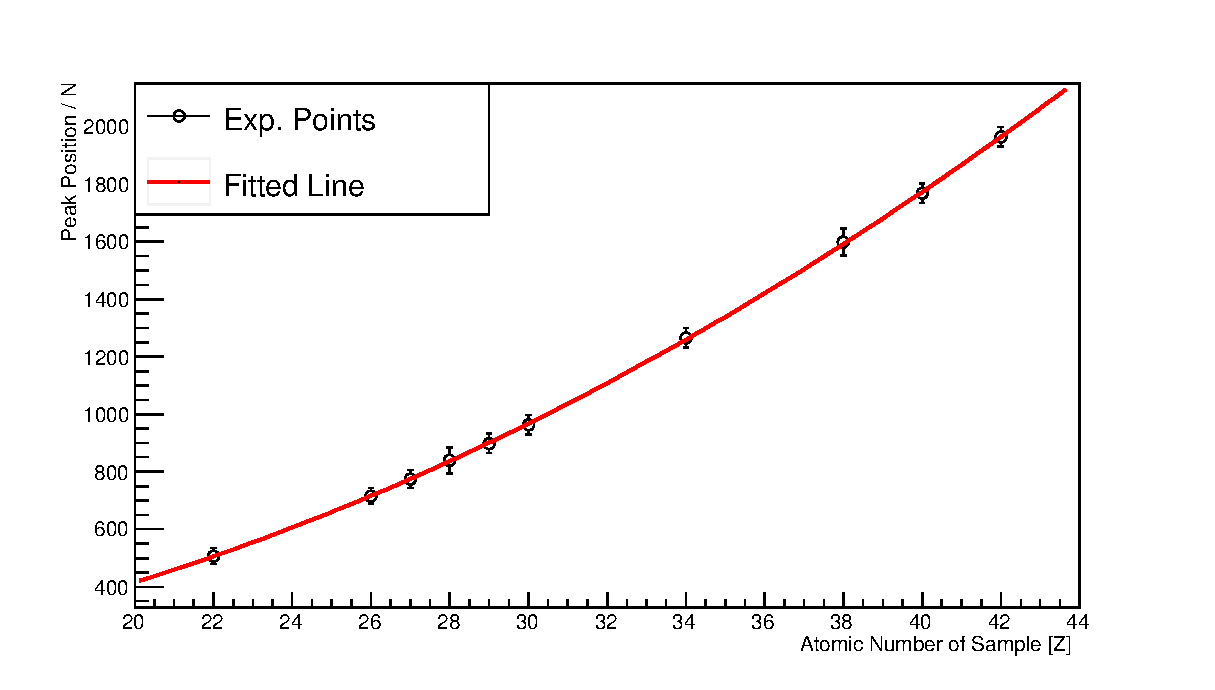
\includegraphics[width=\textwidth]{c1.eps}
\caption{\label{fig:res}%
    莫塞莱定律验证实验的实验数据图像与拟合曲线图像.拟合采用的公式为式~\ref{eq:relation},
    拟合结果为$p_0 = 1.26678, p_1 = 3.20796, p_2 = 58.4646, EDM =
    \num{1.0241e-06},
    \chi^2 = 0.108221$
}
\end{figure}

通过图线和拟合数据可以看出,莫塞莱定律在本实验中得到了较为精确的验证.

\subsection{X射线的吸收}

对于X射线的吸收特性的实验,实验数据如表格~\ref{tab:data2}所示.

\begin{table}[htbp]
  \caption{\label{tab:data2}
      X射线吸收特性的测量实验结果表,表中计数率即为峰下的平均每秒计数,单位为计数/
      秒.
  }
\begin{ruledtabular}
  \begin{tabular}{llllll}
      Al片层数 & 0 & 2 & 4& 6& 8 \\
      Mo谱峰计数率 &98.49 & 31.20 &14.32&11.02&6.68 \\
    \colrule
      Al片层数 & 0 & 2 & 4& 6& 8 \\
      Sr谱峰计数率 &384.32 & 83.59 &21.37&16.41&4.92 \\
      \colrule
      Al片层数 & 0 & 2 & 4& 6& 8 \\
      Se谱峰计数率 &484.01 &42.31 &12.37 &3.34 &0.75 \\
      \colrule
      Al片层数 & 0 & 1 & 2& &  \\
      Fe谱峰计数率 &205.35 &2.86 &0.46 & & \\
      \colrule
      Al片层数 & 0 & 1 & 2& 3 & 4  \\
      Zn谱峰计数率 &438.77 &41.38 &12.33 &5.66 &1.29 \\
      \colrule
      Al片层数 & 0 & 1 & 2&3 &  \\
      Ni谱峰计数率 &310.75 &5.89 &3.49 &0.95 & 
\end{tabular}
\end{ruledtabular}
\end{table}

对于实验数据的初步分析表明,实验结果对于X射线的指数吸收率的偏离较远,并不能用以验
证吸收介质吸收X射线的指数吸收率.分析表明,这是因为实验使用的硅探测器探头大小太小,
导致在测量中的峰计数率严重受到吸收片和样品的摆放位置影响,从而引入过大的误差,使得
测量失去了意义.

\section{结论}

实验成功地验证了莫塞莱定律所指出的原子的标识X射线频率的平方根和原子序数之间的线
性关系,但未能对于X射线在吸收介质中的吸收规律作出有意义的实验测量.
 
\section{致谢}

感谢王思广老师在实验中认真而专业的指导.
 
\begin{thebibliography}{}
\bibitem{Book} 吴思成,王祖铨~2010 近代物理实验(第三版)(北京:高等教
育出版社)第29页.
\end{thebibliography}
 
\clearpage
\appendix
 
\section{代码}

本实验中的实验数据处理使用了Cern开发的ROOT数据分析框架软件,数据分析的相关代码附
在了文后.

\lstinputlisting[language=C++]{analyze.C}
 
\end{document}
